\documentclass[letterpaper,10pt]{article}
\usepackage[top=2cm, bottom=1.5cm, left=1cm, right=1cm]{geometry}
\usepackage{amsmath, amssymb, amsthm,graphicx}
\usepackage{fancyhdr}
\pagestyle{fancy}

\lhead{\today}
\chead{MATH 710 Assignment 6}
\rhead{Justin Hood}

\newcommand{\Z}{\mathbb{Z}}
\newcommand{\Q}{\mathbb{Q}}
\newcommand{\R}{\mathbb{R}}
\newcommand{\C}{\mathbb{C}}
\newtheorem{lem}{Lemma}

\begin{document}
\begin{enumerate}
\item We consider the problem, of solving
\[Ax=b\]
where we require $A^{-1}$. This computation is intensive, so we wish to approximate $A^{-1}$ by solving the problem,
\[By=x\]
Where $B$ is our goal. As a measure of error, we consider the MSE formula,
\[MSE=\sum(y-\hat{y})^2/N\]
Here,
\[MSE=\sum(By-x)^2/N\]
Which may be computed as the L2 norm of the vector, $<By-x>$.\\\\
The results of this attempt are contained in the python notebook for this assignment.
\item We consider the data points, $(0,2),\ (\frac{\pi}{2},1),\ (\pi,3),\ (\frac{3\pi}{2},2)$. In order that we might fit the data to the function,
\[y=c_0+c_1\cos(x)+c_2\sin(x)+c_3\cos(2x)\]
we must consider the following matrix equation, $f(X)\vec{C}=\vec{Y}$, where $f(X)$ is the matrix of coefficients from the desired equation. This equation is then,
\[f(X)=\begin{bmatrix}
1 & \cos(x_1) & \sin(x_1) & \cos(2x_1) \\
1 & \cos(x_2) & \sin(x_2) & \cos(2x_2) \\
1 & \cos(x_3) & \sin(x_3) & \cos(2x_3) \\
1 & \cos(x_4) & \sin(x_4) & \cos(2x_4)
\end{bmatrix}=\begin{bmatrix}
1 & 1 & 0 & 1 \\
1 & 0 & 1 & -1 \\
1 & -1 & 0 & 1 \\
1 & 0 & -1 & -1
\end{bmatrix}\]
From this, we arrive at the matrix equation,
\[\begin{bmatrix}
1 & 1 & 0 & 1 \\
1 & 0 & 1 & -1 \\
1 & -1 & 0 & 1 \\
1 & 0 & -1 & -1
\end{bmatrix}\begin{bmatrix}
c_0\\
c_1\\
c_2\\
c_3
\end{bmatrix}=\begin{bmatrix}
2\\
1\\
3\\
2
\end{bmatrix}\]
In order that we might solve this, we numerically use \textit{numpy} to compute the solution directly from matrix inversion. Thus, we arrive at the equation,
\[y=2-\frac{1}{2}\cos(x)-\frac{1}{2}\sin(x)+\frac{1}{2}\cos(2x)\]
Fitting this equation and overlaying the data, we see the following plot,
\begin{center}
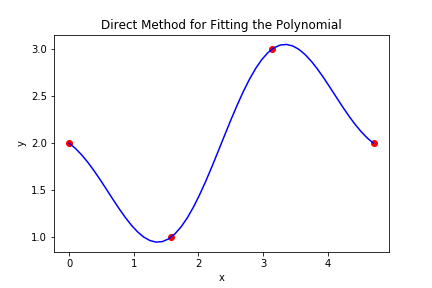
\includegraphics[scale=1]{2.png}
\end{center}
\item In our notebook, we are given data called, ``Even-Data", working under the assumption that this data is truly from an even function, we will use a Discrete Cosine Transform. We begin by assuming that the data is over the interval $x\in [-\pi,\pi]$. Thus, we construct a set of $x$ values that cover this range with the same number of points as the sample data. We then apply our DCT to the data and plot the results over the functional data as follows,
\begin{center}
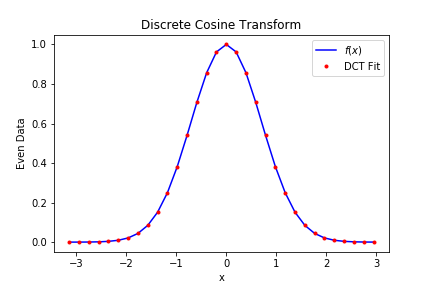
\includegraphics[scale=1]{3.png}
\end{center}
\item In the above problem, we computed the DCT using all 32 points, arriving at an interpolating function from 32 frequencies. We compute the normalized frequencies and plot the results,
\begin{center}
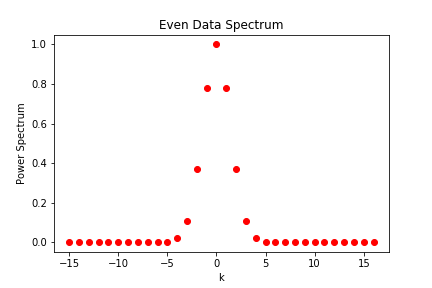
\includegraphics[scale=1]{EvenPower.png}
\end{center}
We see that the relative coefficient powers are mostly negligible save for a few, so we consider reconstructing the data using only the ``important" coefficients. We consider the two cases below, where the cutoff for power is $0.2$ and $0.5$.
\begin{center}
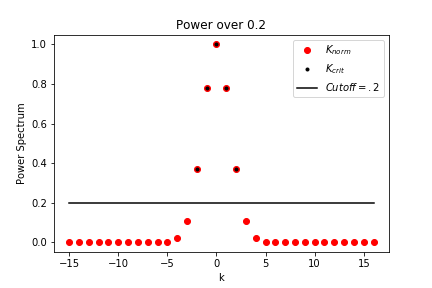
\includegraphics[scale=.5]{32.png}
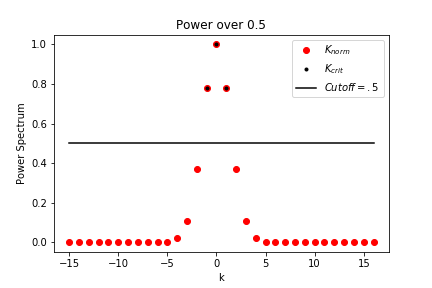
\includegraphics[scale=.5]{35.png}
\end{center}
By reconstructing the DCT with only the ``important" coefficients, we arrive at the following reconstructions,
\begin{center}
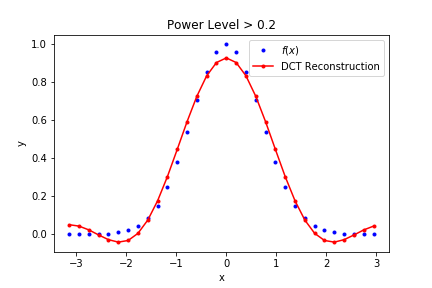
\includegraphics[scale=.5]{32reconstruct.png}
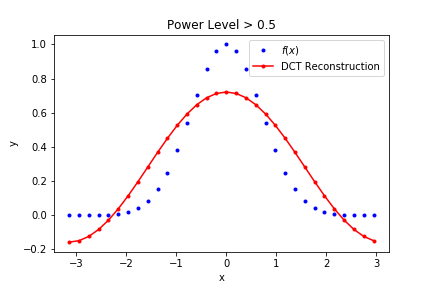
\includegraphics[scale=.5]{35reconstruct.png}
\end{center}
We see that both reconstructions are fairly close to the true data, but the lower cutoff value does have better reconstructive accuracy.
\item Next, we will apply a similar approach to problem 3, but using the DST instead as this data is odd. The resultant reconstruction is,
\begin{center}
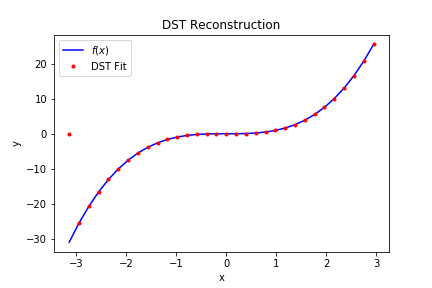
\includegraphics[scale=.75]{5.png}
\end{center}
We see that the left most value of the reconstruction is incorrect, but this is merely because we have reconstructed the data as,
\[f(x)=\sum b_n\sin(kx)\]
In this model, there is no constant value, and since $\sin(n\pi)=0$, the value at the edges of the interval, $x\in[-\pi,\pi]$, our DST risks inaccuracy. If we chose to ignore the edge points, we would see that the interpolated data is more accurate.
\item We now consider the Pallas Asteroid data from Gauss. The data was collected over the range $0$ to $330$ degrees. We begin by performing a standard DCT and DST on the data, as in problems 3 and 5. We then reconstruct the data as the sum of the DCT and DST. The resultant reconstruction is,
\begin{center}
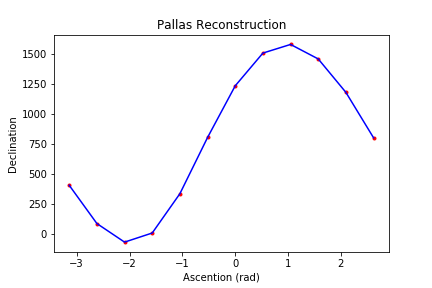
\includegraphics[scale=.75]{6.png}
\end{center}
We see that this reconstruction is quite accurate, but requires a high number of frequencies in both the DST and DCT. Thus, we consider what would happen if we reconstructed the signal using less frequencies.
\item Computing the power spectrums for both the DCT and DST, and finding the cutoff for frequency importance, we arrive at the following important frequencies,
\begin{center}
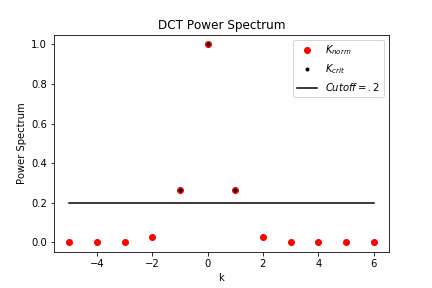
\includegraphics[scale=.5]{7a.png}
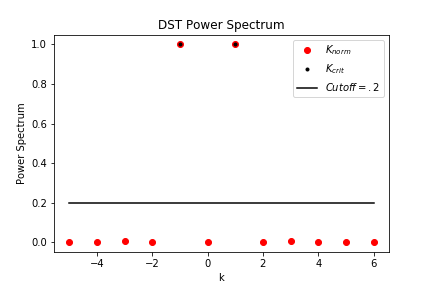
\includegraphics[scale=.5]{7b.png}
\end{center}
Hence, we see that there are 3 important frequencies for the DCT and 2 for the DST. So, we reconstruct the function as, 
\[r(\theta)=a_{k^*_1}\cos(k^*_1\theta)+a_{k^*_2}\cos(k^*_2\theta)+a_{k^*_3}\cos(k^*_3\theta)+b_{k^*_1}\sin(k^*_1\theta)+b_{k^*_2}\sin(k^*_2\theta)\]
This is in essence the sum of critical values for DST and DCT values. Using this functional model, we reconstruct the function over the interval,
\begin{center}
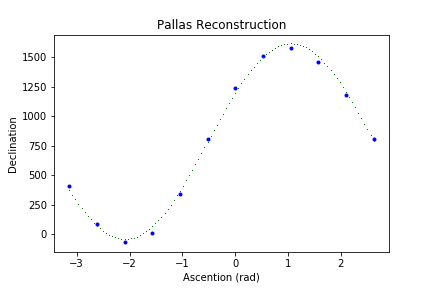
\includegraphics[scale=1]{7.png}
\end{center}
We see that this reconstruction is surprisingly accurate considering it only uses a total of $5$ frequencies.
\item We shall now prove orthogonality as follows.
\begin{equation}
\frac{1}{L}\int_{-L}^L\cos(2\pi \frac{m}{L} x)\cos(2\pi \frac{n}{L} x)dx
\end{equation}
First, we use the cosine sum/product rule to expand the integrand,
\begin{align*}
cos(2\pi \frac{m}{L} x)\cos(2\pi \frac{n}{L} x) &= \frac{1}{2}\bigg(\cos(2\pi \frac{m}{L} x+2\pi \frac{n}{L} x)+\cos(2\pi \frac{m}{L} x-2\pi \frac{n}{L} x)\bigg)\\
&=\frac{1}{2}\bigg(\cos(2\pi \frac{m+n}{L} x)+\cos(2\pi \frac{m-n}{L} x)\bigg)
\end{align*}
Our integral then becomes,
\[\frac{1}{2L}\int_{-L}^L\bigg(\cos(2\pi \frac{m+n}{L} x)+\cos(2\pi \frac{m-n}{L} x)\bigg)dx\]
Then, we shall set $m=n$ and integrate,
\begin{align*}
\frac{1}{2L}\int_{-L}^L\bigg(\cos(2\pi \frac{m+n}{L} x)+\cos(2\pi \frac{m-n}{L} x)\bigg)dx &= \frac{1}{2L}\int_{-L}^L\bigg(\cos(2\pi \frac{2m}{L} x)+\cos(0)\bigg)dx\\
&= \frac{1}{2L}\int_{-L}^L\bigg(\cos(2\pi \frac{2m}{L} x)+1\bigg)dx\\
&= \frac{1}{2L}\bigg(\int_{-L}^L\cos(2\pi \frac{2m}{L} x)dx+\int_{-L}^L1dx\bigg)\\
&=\frac{1}{2L}\bigg(\frac{L}{4\pi m}\sin(2\pi \frac{2m}{L} x)\bigg|_{-L}^L+2L\bigg)\\
&=\frac{1}{2L}\bigg(0+2L)\\
&=1
\end{align*}
Next, we consider $m\neq n$. The integral then becomes,
\begin{align*}
\frac{1}{2L}\int_{-L}^L\bigg(\cos(2\pi \frac{m+n}{L} x)+\cos(2\pi \frac{m-n}{L} x)\bigg)dx &= \frac{1}{2L}\bigg(\frac{L}{2\pi(m+n)}\sin(2\pi \frac{m+n}{L} x)\bigg|_{-L}^L+\frac{L}{2\pi(m-n)}\sin(2\pi \frac{m-n}{L} x)\bigg|_{-L}^L\bigg)\\
&=0
\end{align*}
Thus, have that the solution,
\[I=\begin{cases}
1 & m=n\\
0 & m\neq n
\end{cases}=\delta_{mn}\]
As desired. Next, we consider the integral,
\begin{equation}
\frac{1}{L}\int_{-L}^L\sin(2\pi \frac{m}{L} x)\sin(2\pi \frac{n}{L} x)dx
\end{equation}
First, we use the cosine sum/product rule to expand the integrand,
\begin{align*}
\sin(2\pi \frac{m}{L} x)\sin(2\pi \frac{n}{L} x) &= \frac{1}{2}\bigg(\cos(2\pi \frac{m}{L} x-2\pi \frac{n}{L} x)-\cos(2\pi \frac{m}{L} x+2\pi \frac{n}{L} x)\bigg)\\
&= \frac{1}{2}\bigg(\cos(2\pi \frac{m-n}{L} x)-\cos(2\pi \frac{m+n}{L} x)\bigg)
\end{align*}
Our integral then becomes,
\[\frac{1}{2L}\int_{-L}^L\bigg(\cos(2\pi \frac{m-n}{L} x)-\cos(2\pi \frac{m+n}{L} x)\bigg)dx\]
Then, we shall set $m=n$ and integrate,
\begin{align*}
\frac{1}{2L}\int_{-L}^L\bigg(\cos(2\pi \frac{m-n}{L} x)-\cos(2\pi \frac{m+n}{L} x)\bigg)dx &= \frac{1}{2L}\int_{-L}^L\bigg(\cos(0)-\cos(2\pi \frac{2m}{L} x)\bigg)dx\\
&=\frac{1}{2L}\int_{-L}^L\bigg(1-\cos(2\pi \frac{2m}{L} x)\bigg)dx\\
&=\frac{1}{2L}\bigg(2L-\frac{L}{4m\pi}\sin(2\pi \frac{2m}{L} x)\bigg|_{-L}^L\bigg) \\
&=\frac{1}{2L}\bigg(2L-0\bigg)\\
&=1
\end{align*}
Next, we consider $m\neq n$. The integral then becomes,
\begin{align*}
\frac{1}{2L}\int_{-L}^L\bigg(\cos(2\pi \frac{m-n}{L} x)-\cos(2\pi \frac{m+n}{L} x)\bigg)dx &= \frac{1}{2L}\bigg(\frac{L}{2\pi (m-n)}\sin(2\pi \frac{m-n}{L} x)\bigg|_{-L}^L-\frac{L}{2\pi (m+n)}\sin(2\pi \frac{m+n}{L} x)\bigg|_{-L}^L\bigg)\\
&=0
\end{align*}
Thus, we have the solution as,
\[I=\begin{cases}
1 & m=n \\
0 & m\neq n
\end{cases}=\delta_{mn}\]
As desired. Finally, we consider the integral,
\begin{equation}
\frac{1}{L}\int_{-L}^{L}\cos(2\pi \frac{m}{L}x)\sin(2\pi\frac{n}{L}x)dx
\end{equation}
First, we use the cosine sum/product rule to expand the integrand,
\begin{align*}
cos(2\pi \frac{m}{L}x)\sin(2\pi\frac{n}{L}x) &= \frac{1}{2}\bigg(\sin(2\pi \frac{m}{L}x+2\pi\frac{n}{L}x)-\sin(2\pi \frac{m}{L}x-2\pi\frac{n}{L}x)\bigg)\\
&= \frac{1}{2}\bigg(\sin(2\pi \frac{m+n}{L}x)-\sin(2\pi \frac{m-n}{L}x)\bigg)
\end{align*}
Our integral then becomes,
\[\frac{1}{2L}\int_{-L}^{L}\bigg(\sin(2\pi \frac{m+n}{L}x)-\sin(2\pi \frac{m-n}{L}x)\bigg)dx\]
Setting $m=n$ and integrating, we find,
\begin{align*}
\frac{1}{2L}\int_{-L}^{L}\bigg(\sin(2\pi \frac{m+n}{L}x)-\sin(2\pi \frac{m-n}{L}x)\bigg)dx &= \frac{1}{2L}\bigg(\frac{L}{2\pi (m+n)}\cos(2\pi \frac{2m}{L}x)\bigg|_{-L}^L-0\bigg)\\
&= \frac{1}{2L}\bigg(\frac{L}{2\pi (m+n)}(\cos(4\pi m)-\cos(-4\pi m))-0\bigg)\\
&= 0
\end{align*}
Next, we consider $m\neq n$ and integrate,
\begin{align*}
\frac{1}{2L}\int_{-L}^{L}\bigg(\sin(2\pi \frac{m+n}{L}x)-\sin(2\pi \frac{m-n}{L}x)\bigg)dx &= \frac{1}{2L}\bigg(\frac{L}{2\pi (m+n)}\cos(2\pi \frac{m+n}{L}x)\bigg|_{-L}^L-\frac{L}{2\pi (m-n)}\cos(2\pi \frac{m-n}{L}x)\bigg|_{-L}^L\bigg)\\
&= \frac{1}{2L}\bigg(\frac{L}{2\pi (m+n)}(\cos(4\pi (m+n))-\cos(-4\pi (m+n))\\
&-\frac{L}{2\pi (m-n)}(\cos(4\pi (m-n))-\cos(-4\pi (m-n))\bigg)\\
&= 0
\end{align*}
Noting that $m-n\in \Z$, we may easily reduce the trigonometric fuctions to $1$'s and $0$'s for easy integrating. So,
\[I=\begin{cases}
0 & m=n\\
0 & m\neq n
\end{cases}=0\]
As desired.
\item We now consider,
\[\frac{1}{2\pi}\int_{-\pi}^{\pi}f(x)\cos(kx)dx, \text{ f odd}\]
If $f(x)$ is an odd function, we may state,
\[f(-x)=-f(x)\]
So consider,
\[g(x)=f(x)\cos(kx)\]
Then,
\begin{align*}
g(-x) &= f(-x)\cos(-kx) \\
&= (-f(x))(\cos(kx))\\
&= -g(x)
\end{align*}
So, $g(x)$ is an odd function. As proven before, we know that the integral of an odd function over a symmetric interval is $0$. So,
\[\frac{1}{2\pi}\int_{-\pi}^{\pi}f(x)\cos(kx)dx=0\]
As desired.\\
We now consider,
\[\frac{1}{2\pi}\int_{-\pi}^{\pi}f(x)\sin(kx)dx, \text{ f even}\]
If $f(x)$ is an even function, we may state,
\[f(-x)=f(x)\]
So consider,
\[g(x)=f(x)\sin(kx)\]
Then,
\begin{align*}
g(-x) &= f(-x)\sin(-kx) \\
&= (f(x))(-\sin(kx))\\
&= -g(x)
\end{align*}
So, $g(x)$ is an odd function. As proven before, we know that the integral of an odd function over a symmetric interval is $0$. So,
\[\frac{1}{2\pi}\int_{-\pi}^{\pi}f(x)\sin(kx)dx=0\]
As desired.
\end{enumerate}
\end{document}
